\documentclass{article}
\usepackage{graphicx}
\usepackage[utf8]{inputenc}

\title{7g rapport}
\author{Henrik Flindt\\Nicolas Dyhrman\\Adrian Joensen}
\date{\today}

\begin{document}
    \maketitle
    \section{Manual}
    Awari (or as it is called in its original tongue Oware) is a game in the Mancala family of board games played through out the world. To play the game by double clicking playAvari.exe. Player 1 goes first. The player must select a row between 1-6 that contain more than zero beans. For more rules about the game see https://en.wikipedia.org/wiki/Oware
    
    \section{Design}
        As part of the game development assigment it war required that the programming paradigm "Functional programming" was used. To ensure that the distribution of the beans on the board would be consistent and easily transformed between different functions it was decided to keep the board as an abstract form in a list. 
        Visually, it was decided a command prompt (CMD) as the user interface insted of developing an actual graphic user interface. 
        

    \section{Implementation}
        As part of the assigment a libary was given. While some of these functions were directly implemented as intented, some were modified, or removed. Through out the source code there are several print statments that are commented out. These are left deliberately as they serves as a great aid in debugging. A few extra functions were also implemented when required. While there are 13 functions in all, only those deemed non-trivial is explained in its full.\newline To see the full source code, see last part of this rapport. A brief overview is show below in their occurring order. \newline         
        \textbf{clearPit (l: int list) p}
         Clears the element that corresponds to the chosen pit in the list.\newline
         \textbf{matchOppsitePit (p: pit): pit }\newline
                Returns the opposite pit number as in realation to the indexes of the board list. To ensure that the compiler would compile with no warnings, an default function was added.  \newline 
        \textbf{emptyPit (b: board) (p: pit) : board * pit }\newline
                The most technically advanced move in Awari is the zero-steal move. If a bean lands in a empty pit the \verb|distribute| calls this function. Depending upon what player makes the zero-steal move, the function creates several small lists containing the pits values before and after the pit p containing zero, and the opposition pit op (This value is returned from \verb|matchOppsitePit|). Finally all these small list are truncated and returned.  \newline
         \textbf{ rec distribute (l: board) (p : pit) (b : int) (player : player) : board * pit }\newline
        Creates a new board list where the pit selected by the player is set to zero, and based upon how many beans it did contain increments the subsequent pits with 1. It a important if check to ensure that a hit to an empty pit will trigger the zero-steal move. It also checks that the move is not done to the players home pit!\\
        If the p value passes the end of the list, distribute is recursively called to let the beans be distrusted around the board.\newline
         \textbf{ printBoard(b: board): unit }\newline
         Prints the board. Several minor charchters are added to aid the understanding og how the game works. Each pit is separated by "$|$", an arrow shows the way the game is played, and "Awari" for style. Due to the way the print function works combined with how the list is oriented in the board, the spacial locality principle is violated, but this is not considered a problem with such a short list.\newline 
         \textbf{ findWinner (b : board) : string }\newline
        Takes the elements that correspond to the players' homes and checks who had won, or an potential draw. It is at the time of writing not been possible to play a "natural" game resulting in a draw. \newline
         \textbf{ isGameOver (b : board) : bool }\newline
        Returns true if either side is empty. (i.e if board list [1..6] or [8..13] has the sum zero)\newline
         \textbf{ isHome (b : board) (p : player) (i : pit) : bool }\newline
            Checks if the player is on his home pit.\newline
         \textbf{ pitEmpty (b:board)(i:int)(x:pit): pit }\newline
Checks if a selected pit is empty, by checking the sum of board list at that index is zero. If so returns a -1.\newline
         \textbf{ reverseNumbers(i:int): int }\newline
Takes a number given by the user and revers its to match the internal list. \newline
         \textbf{ getMove (b : board) (p:player) (q:string) : pit }\newline
            Receives the players' input from the CMD and check if it is a legit move. (i.e. not empty and withing the range of 1-6)\newline
         \textbf{ turn (b : board) (p : player) : board}\newline
           	 Checks controls that the turn changes between player one and two, and calls the repeat function if the move is illegal. \newline
         \textbf{ rec repeat (b: board) (p: player) (n: int) (t : bool) : board}\newline
Makes a large amount of calls to ensure that the game is over and if the moves being done is legal.\newline
        \textbf{play:}\newline
        The main function that gets passed the staring board. This function is allows a to make large effective tests of all the parts at once. \newline
         
    	\section{White Box Testing}
   		The whitebox testing was done eighter by testing specific functions isolated, or by calling \verb|play| but with special case board to see how the code reacted to specific inputs. (4 different win conditions and two draw conditions.) The different outputs are shown with each test here. 
   		To run a test compile the library and the test. Then run the test. 
   		\textbf{clearPit test}\newline
        \verb|clearPit| is checked if it empties the element of the list if index 1, 3, 7 or 13 is given.\\
        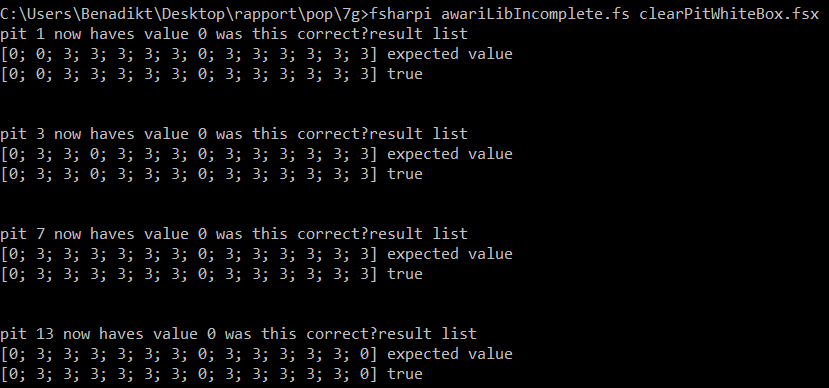
\includegraphics[scale=0.6]{clearPitWhieBox.png}
        \\
          \textbf{win condition check}\newline
        Here a boolean return is checks if it is the correct winner. 
        \\
        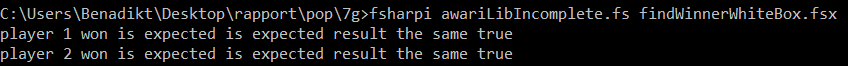
\includegraphics[scale=0.587]{findWinnerWhiteBox.png}
        \\
        \textbf{game over check}\newline
        A series of true-false checks of the \verb|gameOver| 
        \\
        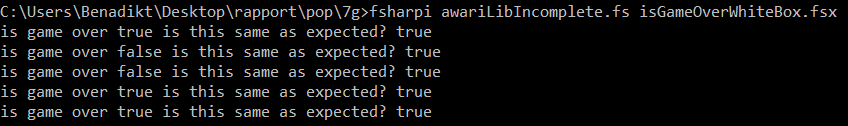
\includegraphics[scale=0.587]{isGameOverWhiteBox.png}
        
        \newpage
        \textbf{distribute check}\newline
        For \verb|distribute| it was check if the function did the arithmetic correct remaining beans (bolds left) from the right place(pit)
        \\
        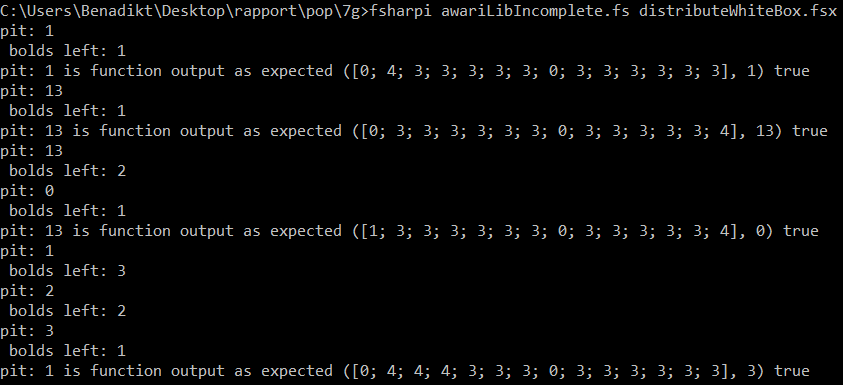
\includegraphics[scale=0.59]{distributeWhiteBox.png}
        \\
      
         
     
        \textbf{isHome check}\newline
       A series of checks going through the different output of \verb|isHome| function. 
        \\
        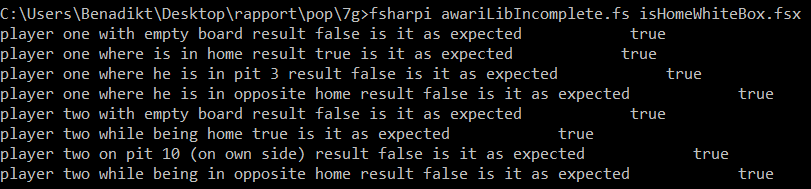
\includegraphics[scale=0.613]{isHomeWhiteBox.png}
        \\
 
        \textbf{getMove check}\newline
        Differet checks based upon user input and if they return the correct response. 
        \\
        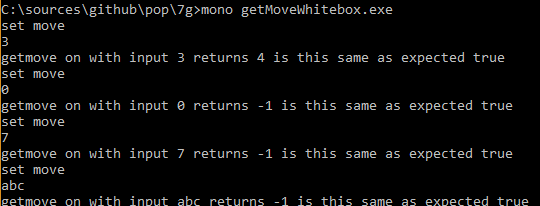
\includegraphics[scale=0.5]{getMoveWhiteBox.png}
        \newpage
        
        \textbf{emptyPit check}\newline
        Checks that the function \verb|emptyPit| returns correct if the players land on an empty pit.
        \\
        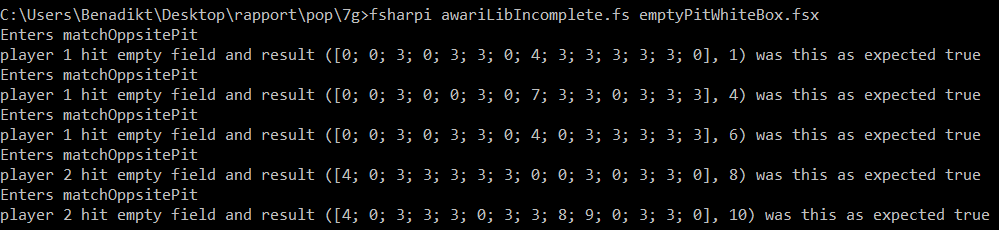
\includegraphics[scale=0.5]{emptyPitWhiteBox.png}
        \\
         \textbf{reverseNumber check}\newline
        Checks if the correct reversed numbers are returned.
        \\
        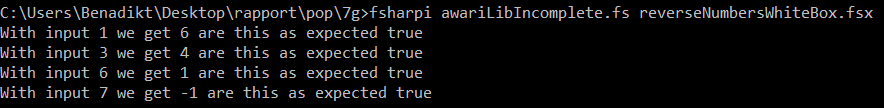
\includegraphics[scale=0.565]{reverseNumbersWhiteBox.png}
        \\
        
         \textbf{pitEmpty check}\newline
        second last it was checked if a empty pit can be selected. 
        \\
        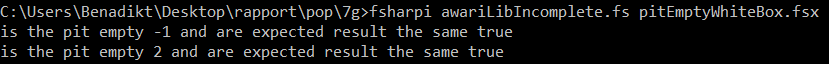
\includegraphics[scale=0.6]{pitEmptyWhiteBox.png}
        \\
        \textbf{Large game test check}\newline
        Finally a large test was done to check if most functions could pass arguments. This was done by passing different boards lists to the \verb|play| and monitor outputs. 
         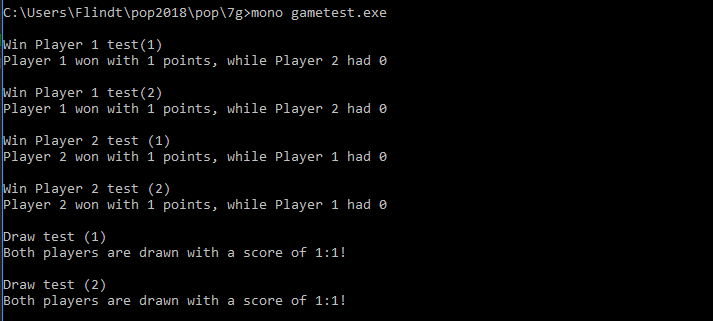
\includegraphics[scale=0.7]{gameTest.png}
      \newline
      
      All tests passed the tests given in the end. 
      
      \section{Black Box testing}
      While no requirements for black box testing was in the assignment, this was indirectly done by playing the game. No issues appeared upon beta testing. 
 
        
        \section{Conclusion}
        Visually the screen was a little difficult to distinguish since the CMD is not an ideal interface for games, and the usage of a list that had a mismatch with the board and user input options, caused quit a large amount of grief. While developing a graphic user interface would have required more code and testing, the amount of work potentially saved debugging errors with a list that mismatch with the user input would potentially have been worth the effort. A  large set of whitebox testing indicates that code functions as required. Potential bugs will most likely be fixed by the Awari modding community.
    \section{Source Code}
    \begin{verbatim}
module Awari
type pit = int
type board = int list
type player = Player1 | Player2


let clearPit (l: int list) p =
let a = l.[0..p-1]
let b = [0]
let c = l.[p+1..13]
a @ b @ c

let matchOppsitePit (p: pit): pit =
//printfn "Enters matchOppsitePit"
match p with
| 1 -> 13
| 2 -> 12
| 3 -> 11
| 4 -> 10
| 5 -> 9
| 6 -> 8
| 8 -> 6
| 9 -> 5
| 10 -> 4
| 11 -> 3
| 12 -> 2
| 13 -> 1
| _ -> -1

let emptyPit (b: board) (p: pit) (player: player): board * pit =
//printfn "Enters emptyPit"
if player = Player1 then 
let op = matchOppsitePit p
//printfn "Exit matchOppesitePit"
let a = b.[..p-1]
let c = [0]
let d = b.[p+1..6]
let home = [b.[7]+b.[p]+b.[op]+1]
let f = b.[8..op-1]
let g = [0]
let h = b.[op+1..13]
let uL = a @ c @ d @ home @ f @ g @ h
(uL, p)
else
//printfn "pit id = %i" p
let op = matchOppsitePit p
//printfn "oPpit id = %i" op
//printfn "Exit matchOppesitePit"
let home = [b.[0]+b.[p]+b.[op]+1]
let a = b.[..(op-1)]
let c = [0]
let d = b.[op+1..7]
let e = b.[8..p-1]
let f = [0]
let g = b.[p+1..13]
//printfn "aLength= %i" a.Length
if a.Length < 2 then
let uL = home @ b.[1..2] @ c @ d @ e @ f @ g 
//printfn "%A" uL
//printfn "a.Length %i" uL.Length
(uL, p)
else 
let uL = home @ a.Tail @ c @ d @ e @ f @ g 
//printfn "other.Length %i" uL.Length
(uL, p)

let rec distribute (l: board) (p : pit) (b : int) (player : player) : board * pit =
let a = l.[..p-1]
let d = [l.[p]+1]
let c = l.[p+1..] //if p = 0 && b = 1 => playerhome + zero pit + obs pit.
if ((l.[p]=0) && (b = 1) && (not (p = 0)) && (not (p = 7))) then
//printfn "pit: %i\n bolds left: %i" p b
emptyPit l p player
else
let uL = a @ d @ c

//printfn "pit: %i\n bolds left: %i" p b

if p >= 13 then
if (b <> 1) then
distribute uL 0 (b-1) player
else
(uL, p)
elif b <= 1 then
(uL, p)
else
distribute uL (p+1) (b-1) player

//printfn "pit: %i\n bolds left: %i" p b



let printBoard(b: board): unit = //For printing the board a variation of the Maurits-printing-metoed seen in previus assigment.
printfn "\n    1   2   3   4   5   6\n           <--         \n    %i | %i | %i | %i | %i | %i\n %i          Awari          %i\n    %i | %i | %i | %i | %i | %i\n" (b.Item(6)) (b.Item(5)) (b.Item(4)) (b.Item(3)) (b.Item(2)) (b.Item(1)) (b.Item(7)) (b.Item(0)) (b.Item(8)) (b.Item(9)) (b.Item(10)) (b.Item(11)) (b.Item(12)) (b.Item(13))
//Spacial locality? What is that...

let findWinner (b : board) : string =
let player1Pit = b.[7]
let player2Pit = b.[0]

if(player1Pit > player2Pit) then
sprintf "Player 1 won with %i points, while Player 2 had %i" player1Pit player2Pit
elif(player1Pit < player2Pit) then
sprintf "Player 2 won with %i points, while Player 1 had %i" player2Pit player1Pit
else sprintf "Both players are drawn with a score of %i:%i!"player1Pit player2Pit



let isGameOver (b : board) : bool =
if b.IsEmpty then
true
else
// checker om player1's side består af 0 pinde
let player2gameover = List.forall (fun elem -> elem = 0) b.[1..6]
// checker om player2's side består af 0 pinde
let player1gameover = List.forall (fun elem -> elem = 0) b.[8..13]

// Returner resultater fra udregninger ovenfor
if player1gameover then
player1gameover
elif player2gameover then
player2gameover
else
false

let isHome (b : board) (p : player) (i : pit) : bool =

// Hvis listen er tom er der ingen hjem derfor return false
if b.IsEmpty then
false
else
// Finder ud af hvor stort halvdelen af boardet er
let halfBoardLen = b.Length / 2

// Plyayer 1's hjem er det første elem (kan også udregnes som 0) men det samme som halvdelen af boardets længde minus halvdelen af boardets længde
let player1Home = halfBoardLen - halfBoardLen

// Player 2's hjem kan udregnes ved at halvere boardets længde (kan også bare laves som halfBoardLen)
let player2Home = b.Length - halfBoardLen

// Checker hvilken spiller der skal tjekkes om er hjemme
match p with
| Player1 ->
if i = 7 then
true
else
false

| Player2 ->
if i = 0 then
true
else
false

let getOppositePit (bLen : int) (i : pit) (p : player) : pit =
match p with
| Player1     -> (bLen / 2) - abs i
| Player2     -> (bLen / 2) + abs i


// pit 1 = player 1's pit
// pit 2 = player 2's pit
let CreateNewBoardFromHitEmptyPit (board : board) (pit1 : pit) (pit2 : pit) (p : player) : board =
printfn "Player 1"

match p with
| Player1 ->
let newHomeValue = board.[7] + board.[pit2] + 1
let a = board.[0 .. (pit1-1)]
let b = [0]
let c = board.[(pit1+1) .. 6]
let d = [newHomeValue]
let e = board.[8 .. (pit2-1)]
let f = [0]
let g = board.[(pit2+1) .. 13]
a @ b @ c @ d @ e @ f @ g

| Player2 ->
let newHomeValue = board.[0] + board.[pit1] + 1
let a = [newHomeValue]
let b = board.[1 .. (pit1-1)]
let c = [0]
let d = board.[(pit1+1) .. 6]
let e = board.[8 .. (pit2-1)]
let f = [0]
let g = board.[(pit2+1) .. 13]
a @ b @ c @ d @ e @ f @ g


let HitEmptyPit (b : board) (i : pit) (p : player) =
if (isHome b p i) then
b
else
let player1 = getOppositePit (b.Length) i Player1
let player2 = getOppositePit (b.Length) i Player2
let newBoard = CreateNewBoardFromHitEmptyPit b player1 player2 p
newBoard


//Checks if a pit is epmty. If so returns -1, else retuns the object pit.
let pitEmpty (b:board)(i:int)(x:pit): pit =
if ((b.Item(i))=0) then  -1 else x;

//Since the board list goes the reveresd of the numbers player one uses, the numbers are matched here.
let reverseNumbers(i:int): int =
match i with
| 1 -> 6
| 2 -> 5
| 3 -> 4
| 4 -> 3
| 5 -> 2
| 6 -> 1
| _ -> -1 //Added to make the compiler stop complaing about unmatched exceptions.

let getMove (b : board) (p:player) (q:string) : pit =
printfn "%s" q

let userInput = System.Console.ReadLine()

let userInt = System.Int32.TryParse(userInput)

match userInt with
| (true, pitValue) ->
if pitValue < 7 && pitValue > 0 then
match p with
| Player1     -> pitEmpty b (reverseNumbers(snd(userInt))) ((b.Length / 2) - abs pitValue)
| Player2     -> pitEmpty b (snd(userInt)+7) ((b.Length / 2) + abs pitValue)
else
-1
| _           -> -1



let turn (b : board) (p : player) : board =

let rec repeat (b: board) (p: player) (n: int) (t : bool) : board =
printBoard b
let str =
if n = 0 then
if t then
sprintf "Invalid user input, please select number between 1 - 6, and be sure that there is one or more beans in the pit. \nPlayer %A's move? " p
else
sprintf "Player %A's move? " p
else
if t then
sprintf "Invalid user input, please select number between 1 - 6, and be sure that there is one or more beans in the pit.\nAgain?"
else
sprintf "Again?"
let i = getMove b p str
if i <> -1 then  //If move is true enteres this loop.

if(i = 13) then //If play2 selects last index in board list.
let (newB, finalPit) = (distribute (clearPit b i) (0) ( b.[i]) p)
if not (isHome b p finalPit) || (isGameOver newB) then
newB
else
repeat newB p (n + 1) false
else
let (newB, finalPit) = (distribute (clearPit b i) (1+i) (b.[i]) p)
if not (isHome b p finalPit) || (isGameOver newB) then
newB
else
repeat newB p (n + 1) false
else
repeat b p n true //If move is false.
repeat b p 0 false

let rec play (b : board) (p : player) : board =
if isGameOver b then
printfn "%s" (findWinner b)
b
else
let newB = turn b p
let nextP =
if p = Player1 then
Player2
else
Player1
//printfn "Before recursive"
play newB nextP


    \end{verbatim}
  
\end{document}
